
%\documentclass[11pt]{article}

%\usepackage{html,latexsym,amssymb,amsmath}




%\title{}

%\date{}

%\begin{document}

%\maketitle


\section{Introduction}\label{SecIntro}

%ecent years, significant progress has been made in the field of
%program verification, in particular in the domain of (sequential)
%smart card
%applications~\cite{BreunesseCHJ03%,JacobsMR04
%}. %However,
%many obstacles still exist that prevent the wide-spread use of these
%techniques. For example, rigorous development methods such as
%refinement~\cite{abrial96,Backrefinement} typically involve the use of
%mathematical specification languages which are difficult for a Java programmer.
%Temporal logics such as LTL (Linear Temporal Logic) and 
%CTL (Computational Tree Logic)~\cite{Em1990} are also far away from the programming language.
%different in kind and
%more difficult to understand than Java code. Similarly, to describe
%the temporal behaviour of a system, one needs complicated logics such
%as LTL (Linear Temporal Logic) and CTL (Computational Tree Logic)~\cite{Em1990}. 
%And to verify that a system adheres to its
%specification the use of automatic techniques such as model
%checking~\cite{ClarkeGP99} is often infeasible, because of the large
%or infinite number of program states, while interactive proving often
%requires expertise with a general purpose theorem prover, such as
%CoQ~\cite{CoqManual96} or B~\cite{abrial96}.


%An interesting development 

Recently, throw the development of the JML
project\footnote{See \texttt{http://www.jmlspecs.org}.},
 significant progresses have been made in the field of
smartcard applications verifications~\cite{BreunesseCHJ03}.
The JML Project defines
a specification language which is syntactically and
semantically closed Java, thus making
specifications more accessible to Java programmers. As part
of the project many tools are developed~\cite{Burdy-etal03}: the JML
tool for runtime assertion checking~\cite{Preliminary}; tools for
program verification, \emph{e.g.}\/~Jack~\cite{BurdyRL03},
ESC/Java2~\cite{CokK04}, Bogor~\cite{bogor2005} 
and Krakatoa~\cite{marche03jlap}; tools for
the generation of annotations such as Daikon~\cite{ErnstCGN01} and
Pavlova's generation method~\cite{Enforcing}. JML allows to add to the
java class traditionnal formal annotations like method 
pre-and postconditions and invariants.% to specify static 
%properties of the class.
%\emph{i.e.,}\/~properties that are preserved by every method in a
%class. 
%Further, it also provides so-called model variables
%(specification-only variables), that provide abstraction %and make the
%language expressive enough 
%to specify the order and conditions under
%which the different methods in a class can be invoked.

%for the purpose of Java code verification is
%the use of JML annotations which are inserted as special comments in
%the code\cite{Enforcing}. These annotations allow the user to specify
%for each method of a class its preconditions-- what must hold before
%the invokation of the method, and its postconditions--what must hold
%after the normal or exceptional termination of the method, and static
%or dynamic (using past value variables) class invariants which must be
%preserved by each method of the class. This language is expressive
%enough to specify the order and conditions in which the methods can be
%invoked. The special use of model variables provides a way of dealing
%with abstract classes making the language powerful enough for code
%verification. This specification language is very useful for
%specifying the functional behavior of the methods since its Java like
%syntax makes it easy to be used by Java software engineers. Moreover,
%it is well instrumented by tools~\cite{Burdy-etal03}. For instance,
%from JML annotations, the tools \textit{Jack} and \textit{ Krakatoa}
%\cite{marche03jlap} allows generating proof obligations which can be
%checked afterwards by dedicated theorem provers such as Coq, PVS,
%atelierB or haRVey \cite{Harvey}. 

Moreover, JML provides so-called \textit{historical constraints}, relying 
value of the variables of the current state with value of the
preceding state, however, it is difficult to directly specify in JML 
more complexe dynamic properties, like liveness properties~\cite{lamport77} 
that are often needed to express the security policies
and behaviors that the Java implementation needs to ensure. 

Take the example of a bank
automaton transaction system  
written in Java\footnote{The ATM specification - \\
\textit{http://www.math-cs.gordon.edu/local/courses/cs211/ATMExample/}}.
Entering the card into the automaton opens 
a new session which stays open until the ejection of the card. During
this session, one can perform several transactions (debit, credit...).
This transaction system  is implemented by a class $Session$
 using instances of the class $Transaction$.
In JML, no structure 
permits to easily expressed the following property on the 
transaction mechanism %further denoted $L$:
\begin{center} 
\textit{``Every transaction must eventually terminates''} 
\qquad ($L$)
\end{center}
For verifying such liveness properties, we propose to introduce a
 \textsf{Loop} operator, closed to 
the Burstall's classical liveness
operator~\cite{burstall}, denoted $Q \leadsto R $ and
 meaning intuitively that  under conditions $Q$ a state where
$R$ holds must \textit{inevitably} be reached.
Using the \textsf{Loop} operator, Property $L$ can be expressed by:
\begin{center}
(\texttt{true}) $\leadsto_{JML}$ (\texttt{state == 6 || state == 7}) $(L_F)$\\
\end{center}
where  the predicate \texttt{state == 6 || state == 7} denotes the end
of the transaction.

This paper propose a method to verify liveness properties expressed by
this  \textsf{Loop} operator on Java application using the JML framework.
%an automatic translation of these properties into standard JML
%annotations.


%This behavior is implemented by a class $Session$ using a class $Transaction$.
%The aim is to verify that the Java implementation 
%ensures the security policies 
%and behaviors described in the specification. 
%Native JML permits already 
%interesting verification possibilities 
%such as checking an invariant, for 
%example:
%\begin{verbatim}
%//@ invariant  pinTry < PIN_MAX_TRY ;
%\end{verbatim}
%This invariant ensures that, in all states, the number of attempts for 
%pin validation, represented by the variable \texttt{pinTry}, must 
%always be lower than the constant \texttt{PIN\_MAX\_TRY}.

%However, to verify security policies, one often need to verify
%liveness properties of a system.  Liveness properties express 
%that, under certain conditions, \textit{``something good'' } will 
%eventually happen~\cite{Lamport77} and are useful, for example,
%to express that an opened channel must eventually be closed, that
%a task in a queue must eventually be done.
%So-far JML does not 
%%natively support that. 
%In JML, no structure 
%permits to easily expressed the following property on the 
%transaction mechanism %further denoted $L$:
%\%begin{center} 
%\textit{``Every transaction must eventually terminates''} 
%\qquad ($L$)
%\end{center}



%In the paper, we help the specifier by proposing
%\begin{enumerate}
%\item a primitive \textsf{Loop} to express liveness properties, denoted $Q \leadsto_{JML} R $, meaning that under conditions $Q$, the state $R$ must
%eventually be reached.
%\item an automatic translation of these properties into standard JML
%annotations implemented into a tool.
%\end{enumerate}

% For example, the liveness property ($L$) can be expressed by the 
%\textsf{Loop} operator.

%This paper addresses this shortcoming by defining a way to verify
%liveness properties that can be expressed by this liveness primitive. 








\begin{figure}[t]
\begin{center}
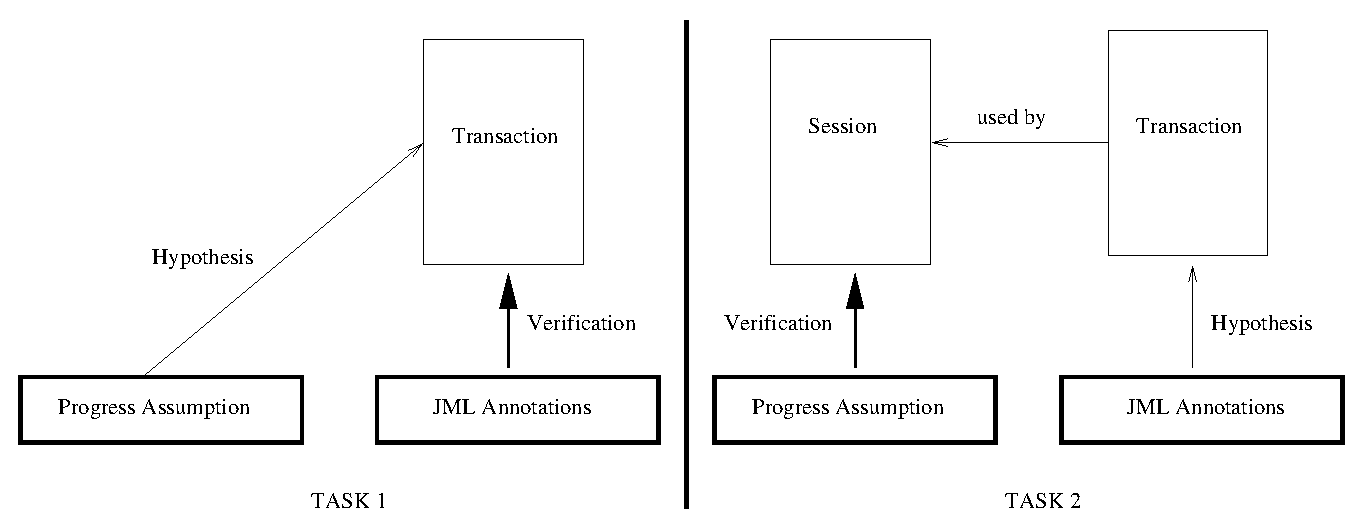
\includegraphics[scale=0.5]{model.eps}
\end{center}
\caption{Verification of Liveness Property: The example of Session and Transaction}

\label{fig-TS}
\end{figure}


%\begin{figure}[t]
%\begin{center}
%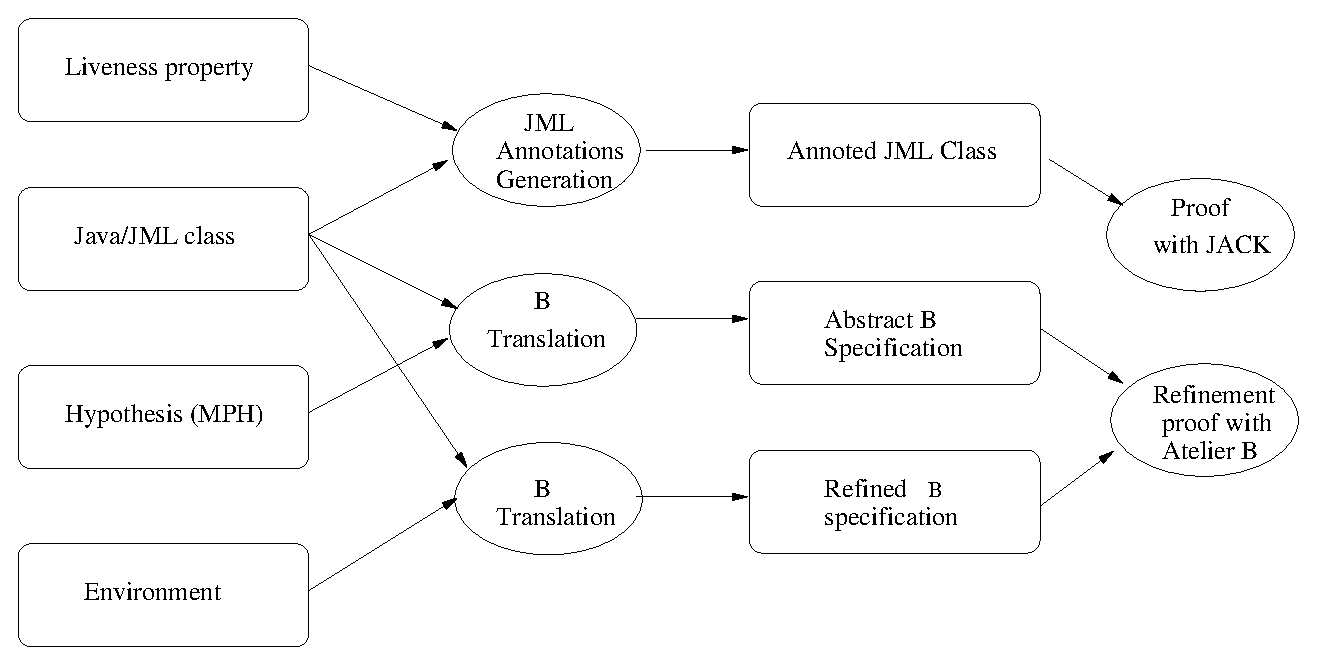
\includegraphics[scale=0.5]{general.eps}
%\end{center}
%\caption{Liveness Verification Method}

%\label{genpe}
%\end{figure}

%Indeed, the property ($L_F$)
%cannot be translated into an invariant.
 To prove a property expressed by the 
\textsf{Loop} operator on the class $Transaction$, 
one need to discover a \textit{variant} 
expression $V$ over a well-founded set. 
Under the condition $Q$,
$V$ must decrease each time a method of $Transaction$ terminates
until the $R$ happens.  %This expression $V$ is usually 
%called a variant. 
Moreover, the surrounding environment of the class, i.e., 
the class $Session$, must also verify some assumption. For example,
we are not able to prove the property ($L$), i.e., that the state 
\texttt{state == 6 || state == 7}
of the class $Transaction$ will eventually be reached, if the 
class $Session$ do not use any instance of $Transaction$. %For that, we need to asssume 
%some \textit{progress} on $Session$ to ensures the verification
%of the temporal property. 
So, to verify the liveness property ($L_F$), 
we need to assume \textit{progress}
on the environment of the class.

%The Figure~\ref{fig-TS} illustrate this problem.
Therefore, we divide the verification of the \textsf{Loop}
operator into two tasks as illustrated in Fig.~\ref{fig-TS}.




%This paper addresses this shortcoming by defining a way to verify
%liveness properties that can be expressed in this JML extension. 
%The basic idea of our approach is to break the verification into two
%different subtasks.  The Figure~\ref{fig-TS} illustrate this example.
\begin{itemize}
\item The first task is to show that, under a \textit{progress}
hypothesis on the environment $Session$, the property expressed by
the \textsf{Loop} operator is verified on the Java class 
$Transaction$, by generating appropriate
JML annotations. Particularly %, when
%$T$ is a liveness, 
one of 
these annotations guarantees that the methods of the class decrease
a variant $V$.  
%When $T$ is a liveness property,
%it is necessary to make some progress assumptions $H$ on the surrounding 
%class $Session$, in the case $T$ is a liveness property. Indeed, 

%Progress of the environment is needed for satisfaction 
%of the liveness properties,
% whereas it is not the case for a safety property. Indeed, according 
%to Lamport~\cite{Lamport77}, a class
%which is not used is always safe -- \textit{``something bad''} will never
%happen since nothing happens. However in general, it does not satisfy liveness %properties.
% Indeed nothing happens,  \textit{``something good''} will never happen.
%Therefore, for the verification of liveness properties, we need a progress 
%assumption $H$ on the environment, i.e., the class \textit{Session}, to 
%establish that $Transaction$ verify the liveness property $T$.

\item %The second task consists in verifying  that the 
%environment, i.e., the class $Session$, preserves the liveness 
%property $T$ when using $Transaction$, i.e., that $Session$
%verifies  the progress. Then $T$ is guaranteed on the whole
%system, i.e., the package $Session$ + $Transaction$.
The second task consists in verifying 
that the environment, i.e., the class $Session$, verify the
\textit{progress} hypothesis. Thus, the liveness property
will be verified on the whole system, i.e., $Transaction$ used by $Session$.
\end{itemize}



%The first subtask is to show that if the class
%\(transaction\) for
%which we wish to show the liveness property is run in an ideal
%environment, \emph{i.e.,}\/~an environment that calls all methods
%sufficiently often, then the liveness property can be established. 
%which  we wish to show the liveness property holds on a class used 
%by an environment under progress hypotheses $H$, then the liveness 
%property can be established. 
%The second subtask is to show that the surrounding system, in which the
%class \(C\) is actually used, preserves the liveness property. 


The paper is outlined as follows. Section~\ref{sec-RunningExample} 
presents JML and the running example.
Section~\ref{sec-temporal} explains liveness verification, 
and we show how to automatically generate JML annotations that are 
sufficient to guarantee liveness properties expressed by the
\textsf{Loop} operator,%defined in~\cite{Huis02},
assuming that the appropriate \textit{progress} assumptions holds on the
environment. We also prove the soundness of the generation.
We have implemented this annoation generation into a tool called \textsf{JAG}.
Section~\ref{sec-verif} presents the second task,
which requires to show that the environment satisfies the progress hypothesis.
The idea is to prove that the class and 
its environment is a liveness-preserving refinement of
the class \(C\) under the \textit{progress} assumption.  %Figure~\ref{genpe}
%depicts the general approach. Notice that instead of proving the JML
%annotations with JACK, they also could be validated using
%any other tool for JML.
Section~\ref{sec-conclusion} concludes and presents 
the perspectives of future work.



